
\begin{figure}[t]
    \centering
    \captionsetup{font=small}
    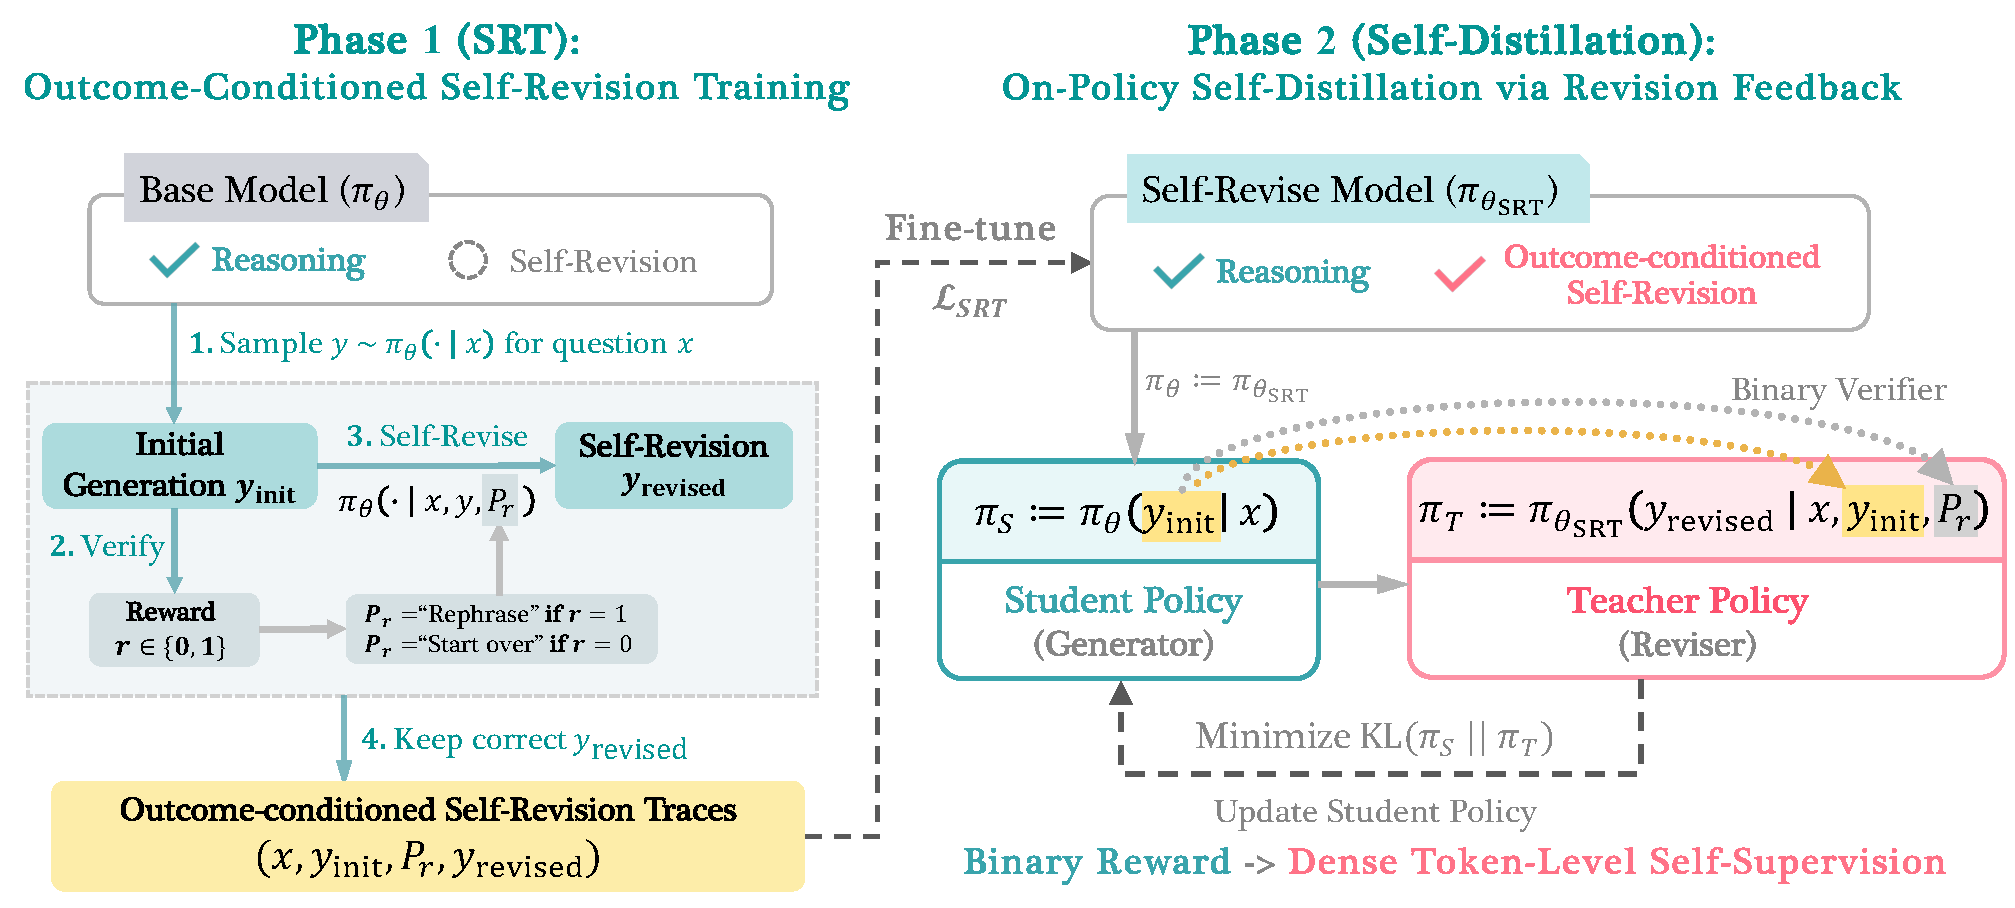
\includegraphics[width=\textwidth]{figures/Picture1.pdf}
    \caption{\textbf{Overview of \ours{}.} In \textbf{Phase 1 (\sft{})}, we collect 6K outcome-conditioned self-revision traces by sampling an initial response from the base model, prompting the model to self-revise its incorrect response, and keeping the correct self-revision. In \textbf{Phase 2 (\opsd{})}, we conduct on-policy self-distillation with the self-revise (\sft{}) model acting as both student and teacher: the \textit{student} generates an on-policy response, and the \textit{teacher} generates a revised version conditioned on that response and its outcome reward. Throughout the \opsd{} phase, the model bootstraps performance through internalizing self-revision behavior. See \Cref{alg:pipeline} for details.
    % \liam{I'm very confused by this diagram - and unless I'm being dumb, I feel like the OPSRD loss setup might not make total sense (notationally)?}
    % \yh{make things consistent with section 2}
    % \\\yj{I'm confused of what are these check signs? So to my understanding, regardless of correctness, the model self-revises the response and filters out only the correct revised response? Also, it's hard to get the fine-tuning objective with this "self-revision traces" and that we are "minimizing" this KL. Finally, I think notations are not consistent with the explanation ($z$ and $y_{revisied}$)?}
    % \danqi{What is $\theta^*$? Do generator and reviser always share weights?}
    }
    
    \label{fig:main-figure}
\end{figure}